% !TeX root = ../../../main.tex
\section{Architektura sieci \textit{Mask R-CNN}}
\label{sec:architekrura_mask_rcnn}

\textit{Mask R-CNN} \cite{matterport-mask-rcnn} (z ang. \textit{Mask Regions with Convolutional Neural Network}) jest implementacją o otwartym kodzie źródłowym modelu do segmentacji instancji opisanego w \cite{general-mask-rcnn}.
W celu zrozumienia tego modelu, najlepiej rozważać go w kontekście ewoluowania kolejnych iteracji, którego końcowym wynikiem jest \textit{Mask R-CNN}.

\subsection{Iteracja pierwsza - \textit{R-CNN}}

\textit{R-CNN} \cite{rcnn} (Rysunek \numberref{fig:r_cnn}) (z ang. \textit{Regions with Convolutional Neural Network}), zaproponowany w 2014 roku, rozwiązuje zagadnienie detekcji obiektów w obrazie (tzn. wskazuje konkretne obiekty, ale bez konkretnych pikseli).

\begin{figure}[h]
  \centering
  \includegraphics[width=1\textwidth]{r-cnn.png}
  \caption{Schemat modelu \textit{R-CNN}}
  \label{fig:r_cnn}
\end{figure}

Działanie tego modelu można zobrazować w następujących krokach:
\label{sec:regiony}
\begin{enumerate}
  \item selekcja regionów zainteresowania z obrazu wejściowego, przy~użyciu algorytmu \textit{Selective Search} \cite{selective-search}, w których prawdopodobnie może znajdować się zanalizowany obiekt;
  \item ekstrakcja cech dla każdego regionu zainteresowania za pomocą \textit{CNN};
  \item klasyfikacja cech wyznaczonych dla regionu przy wykorzystaniu modelu wektorów nośnych; wynikiem tej klasyfikacji jest podział regionów na dwie grupy - zdetektowany obiekt lub niezdetektowany obiekt;
  \item tylko dla regionów ze zdetektowanym obiektem, próba dopasowania obszaru do rozmiaru obiektu, wynikiem czego jest obwiednia (z ang. \textit{bounding box}) wskazująca granice analizowanego obiektu.
\end{enumerate}

\subsection{Iteracja druga - \textit{Fast R-CNN}}
\label{sec:fastrcnn}

\textit{Fast R-CNN} \cite{fast-rcnn} (Rysunek \numberref{fig:fast_r_cnn}), przedstawiony w 2015 roku, jest usprawnieniem modelu \textit{R-CNN} o zoptymalizowaną ekstrakcję cech. 
W modelu modelu \textit{R-CNN} zidentyfikowano następujące problemy:

\begin{itemize}
  \item problem w implementacji i w wytrenowaniu sieci, wynikający z samej budowy \textit{R-CNN}; \textit{R-CNN} składa się z~czterech części, które osobno wymagają zrozumienia, implementacji i~trenowania lub doboru parametrów:
		\begin{itemize}
			\item \textit{Selective Search}, w detekcji regionów zainteresowania,
			\item \textit{CNN}, do ekstrakcji cech dla wyznaczonych regionów,
			\item \textit{SVM}, do klasyfikacji wyekstrahowanych cech,
			\item modelu dopasowującego obwiednię;
		\end{itemize}
  \item zduplikowane obliczenia na etapie ekstrakcji cech dla regionów zainteresowania zachodzących na siebie, co wynika z~faktu, iż ekstracja cech uruchamiana jest dla każdego z regionów, niezależnie od tego czy te regiony zachodzą na siebie.
\end{itemize}

\begin{figure}[h]
  \centering
  \includegraphics[width=1\textwidth]{fast_r-cnn.png}
  \caption{Schemat modelu \textit{Fast R-CNN}}
  \label{fig:fast_r_cnn}
\end{figure}

Wyróżnione na Rysunku \numberref{fig:fast_r_cnn} elementy wskazują zasadnicze różnice względem \textit{R-CNN} (Rys.~\numberref{fig:r_cnn}).

Używając \textit{Fast R-CNN}, ekstrakcja cech następuje następuje tylko raz, na początku procesu.
W ten sposób powstaje mapa cech całego obrazu.
Gdy zachodzi konieczność ekstrakcji cech regionu zainteresowania, zamiast liczyć cechy od nowa, wyciągany jest odpowiadający fragment mapy cech.
Metoda ta to tzw. \textit{Region of Interest Pooling} \cite{fast-rcnn}.

Oprócz zmian w sposobie liczenia cech, w \textit{Fast R-CNN} klasyfikator \textit{SVM} został zastąpiony siecią neuronową.
Podobnie stało się z~modelem dopasowującym obwiednię.
Te dwie nowe sieci połączono w jedną sieć wraz z~siecią \textit{CNN}.
Podsieć klasyfikująca i podsieć dopasowująca obwiednię zostały włączone do sieci w sposób równoległy, tzn. ich wyniki nie zależą od siebie nawzajem.

Zmiany te rozwiązały w dużej części wymienione w punkcie \numberref{sec:fastrcnn} problemy modelu \textit{R-CNN}.

\subsection{Iteracja trzecia - \textit{Faster R-CNN}}

\textit{Faster R-CNN} \cite{faster-rcnn} (Rysunek \numberref{fig:faster_r_cnn}), przedstawiony w 2016 roku, wprowadza usprawnienie dotyczące generowanie regionów zainteresowania za pomocą algorytmu \textit{Selective Search} \cite{selective-search}, który działał stosunkowo wolno.
Usprawnienie polegało na zastąpieniu algorytmu nową siecią neuronową, która korzysta z~cech obrazu do generowania regionów zainteresowania.
Jako że sieć została włączona do modelu w taki sposób, że bazuje na wyznaczonej mapie cech, to uzyskano w ten sposób znacznie szybszy model.
Dodatkowo był to kolejny krok zastępujący część modelu podsiecią neuronową, w wyniku czego model stał się jedną siecią neuronową, składającą się z~podsieci: budującej mapę cech, generującej regiony zainteresowania, klasyfikującej analizowany region oraz dopasowujący obwiednię do zdetektowanego obiektu.

\begin{figure}[h]
  \centering
  \includegraphics[width=1\textwidth]{faster_r-cnn.png}
  \caption{Schemat modelu \textit{Faster R-CNN}}
  \label{fig:faster_r_cnn}
\end{figure}

Wyróżniony na Rysunku \numberref{fig:faster_r_cnn} element wskazuje zasadniczą różnicę względem \textit{Fast R-CNN}, polegającą na zoptymalizowanej metodzie generowania regionów zainteresowania.

\newpage
\subsection{Iteracja czwarta - \textit{Mask R-CNN}}
\label{sec:maskrcnn}
\textit{Mask R-CNN} \cite{matterport-mask-rcnn} (Rysunek \numberref{fig:mask_r_cnn}), przedstawiony w 2017 roku, stanowi ostatni krok w opisanej ewolucji modelu \textit{R-CNN}.
Do dwóch równoległych podsieci - klasyfikującej oraz dopasowującej obwiednię - wprowadza nową, równoległą podsieć odpowiedzialną za detekcję konkretnych pikseli obiektu. Wyróżniony element wskazuje zasadniczą różnicę względem \textit{Faster R-CNN}, polegającej na wprowadzeniu nowej podsieci.

\begin{figure}[h]
  \centering
  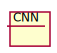
\includegraphics[width=1\textwidth]{mask_r-cnn.png}
  \caption{Schemat modelu \textit{Mask R-CNN}}
  \label{fig:mask_r_cnn}
\end{figure}

Pseudokod \myfigref{alg:mask-r-cnn} przybliża, w jaki sposób powstaje podsieć odpowiedzialna za detekcję maski obiektu.

\begin{algorithm}
  \subimport{}{commoninput}
  \subimport{}{commonoutput}
  \begin{algorithmic}[1]
    \subimport{}{firststepsofmask}
    \State $\mathit{L} \gets [...L,\verb| deconvolution 2x2 with strides 2|]$
    \subimport{}{laststepsofmask}
	\end{algorithmic}
	\caption{Tworzenie podsieci maski}
	\label{alg:mask-r-cnn}
\end{algorithm}
